%%%%%%%%%%%%%%%%%%%%%%%%%%%%%%%%%%%%%%%%%%%%%
\section{Introduction}
\label{sec:intro}
%%%%%%%%%%%%%%%%%%%%%%%%%%%%%%%%%%%%%%%%%%%%%

%% The demand for reliable distributed systems is constantly on the rise.
%% The last two decades have seen a paradigm shift from PC's to SAS and
%% cloud storage. Industrial control systems, and ATM's are naturally
%% distributed applications, which are being implemented at an ever
%% increasing rate. Failures of these systems are frequent and severe,
%% the estimated cost of data centre downtime in 2013 amounted to almost
%% 285 million USD's~\cite{gagnaire2012downtime}.

% JS: The lack of tools is blamed from the start to be a main reason
% for making DS development challenging. Rather, show the reader how
% bad it is to not be able to see global state. Then I would see the
% immediate value of a tool solving it, if it existed. The difference
% is subtle, but I can come up with a long list of things for which
% there are no tools, it doesn't mean that not having the tool is a
% problem.

Developing correct distributed systems remains a formidable challenge. One
reason for this is that developers lack the tools to help them extract
and reason about the distributed state of their
systems~\cite{Ousterhout91therole}.
%
%%  Developers today have few tools to help them extract and reason
%% about distributed state.
The state of a sequential program is well defined (stack and heap),
easy to inspect (with breakpoints) and can be checked for correctness
with assertions.
%
% JS: "The state of a distributed execution is resident across
% multiple nodes and it is unclear how to best compose these states
% into a coherent picture, let alone check it for correctness.".
%
% Can you claim something stronger?  e.g, "The only way to debug a
% distributed system is to compose individual states...". or can you
% list a few quick examples of what one would miss by inspecting one
% node at a time -- (which seems to be, like you claim, the current
% state of affairs)?
%
However, the state of a distributed execution is resident across
multiple nodes and it is unclear how to best compose these states into
a coherent picture, let alone check it for correctness.


%
%% A system on a single machine can be paused with a breakpoint, its
%% state can be inspected, and assert statements can be added to verify
%% certain properties at runtime.
%

In this work we propose a program analyses tool-chain called
\emph{\dinv} for inferring likely data properties, or
invariants, between variables at different nodes in the system.
%
For example, consider a two phase commit protocol in which the
coordinator first queries other nodes for their vote and if all nodes,
including the coordinator, voted ``Commit'' then the coordinator
broadcasts a ``TX Commit'', otherwise it broadcasts a ``TX Abort''. At
the end of this protocol all nodes should either commit or abort. To
check if several non-faulty runs of the system are correct, a
developer can examine the Dinv-inferred distributed state invariants
for this set of executions. In this case they can check whether Dinv
mined the invariant $coordinator.commit = replica_i.commit$ for each
replica $i$ in the system. This would mean that the commit state
across all nodes was identical at consistent snapshots of the system.

Dinv-inferred invariants help developers reason about the distributed
state of their systems in various ways. For
example, they can improve developer understanding of their systems and
confirm expected relationships between variables across the network.
They can also be used by test-case generation techniques to drive the
system towards invalid states (i.e., states that violate an inferred
invariant). These invariants can also help with debugging: a mined
invariant that violates the developer's mental model of what should be
true can be tracked back to observed concrete values, and can be used
to minimize the execution~\cite{scottminimizing}.

Dinv first statically instruments the system's code, either
automatically or with user-supplied annotations. Dinv uses static
program slicing to capture those variables that are affected by or
effect network communication at each node. During system execution,
Dinv instrumentation tracks these variables, collects their concrete
runtime values, tags them with a vector timestamp, and logs the values
at each node. Once the developer has decided that the system has run
long enough (e.g., includes the behavior of interest), they run Dinv
on the generated node logs. Dinv uses these logs to construct a
lattice of distributed states. Our key technical contribution is to
propose three heuristics for merging these distributed states into a
series of system snapshots. Dinv then uses a version of the Daikon
tool~\cite{Ernst07} to infer likely distributed state invariants over
the tracked variables in these snapshots.

%% infer the likely distributed
%% state invariants for the system. These invariants relate variables at
%% different nodes and can be used to check system correctness. For
%% example, in a leader election algorithm Dinv can relate the variable
%% $leader$ at different nodes to derive the invariant
%% $\forall~\textrm{nodes}~i,j,~leader_i == leader_j$. This can increase
%% confidence in the correctness of the system.

%% identify and
%% record at runtime the sets of concrete values for node variables that
%% make up distributed state in a distributed system. It then determines
%% consistent snapshots of distributed state in the system and uses the
%% Daikon tool~\cite{ernst_daikon_tse_2001} to infer likely data
%% relations, or invariants, over the tracked variables.


%for checking distributed systems using and developer comprehension.
%
%In contrast with recent related work~\cite{wilcox_verdi_pldi15,
%  hawblitzel_ironfleet_sosp2015}

Our approach with Dinv is pragmatic: it does not require the developer
to formally specify their system and it scales to large production
systems and long executions. Although Dinv uses dynamic analysis,
which is incomplete (Dinv cannot reason about executions it does not
observe), we believe that it is useful because (1) most distributed
systems developers today use dynamic analysis to check their systems
(e.g., with testing) and (2) we have been able to use Dinv to
validate useful properties in several large systems.

% JS: (1) makes me nervous. you lead your intro by basically saying
% existing tools aren't good. I can only imagine the testing
% methodology reflects the tools available. I think what (1) should
% say is just that dynamic analysis is easy to integrate with test
% frameworks. it doesn't remove anything to say it that way

We evaluated \dinv by using it to study four systems written in Go:
Coreos's etcd~\cite{etcdraft}, Taipei-Torrent~\cite{taipeitorrent},
Groupcache~\cite{groupcache}, and Hashicorp Serf~\cite{serf}. We
targeted different safety and liveness properties in these large
systems and ran Dinv on a variety of executions of each system.  For
example, etcd uses the Raft consensus algorithm~\cite{RaftATC14} and we
checked that the Raft executions we induced satisfy the strong leader
principle, log matching, and leader agreement. We used Dinv over
several iterations to infer distributed state invariants that
confirmed that the executions we studied satisfy each of the targeted
properties. We also report on Dinv's overhead, finding that \dinv can
instrument etcd Raft in a few seconds and that 10 logging annotations
in a Raft cluster of 6 nodes induced a 24\% system
slowdown and 13KB total extra bandwidth on an 30 second
execution.


% I'm reading the last paragraphs of the intro and dissecting it to
% find "claims", "requirements", and "contributions". I'm hoping the
% claims match the eval.
%
% claim 1: Dinv-inferred invariants help developers reason about the
% distributed state of their systems and can be used in a variety of
% ways.
%
% claim 2: ?
%
% requirement 1: no need for developer to formally specify system
%
% requirement 2: scalable both in size of production system (is this
% SLOC, or number of participating nodes?) and duration of execution
%
% contributions are nicely laid out. if you plan on releasing the
% code, say it upfront?

To summarize, this paper makes the following contributions:

\begin{itemize}

\item We propose a method for inferring likely distributed state
  invariants in complex distributed systems. Our method relies on
  well-known program analyses, but combines them in a novel manner.

\item We developed three heuristics for merging distributed node
  states into three kinds of distributed snapshots. We show that each
  heuristic is useful for inferring different types of distributed
  invariants.

\item We describe \dinv, an open source tool that implements the
  proposed method, and evaluate it on several complex Go systems that
  are in widespread use.

\end{itemize}


%% Unlike alternative approaches to verifying
%% distributed systems~\cite{wilcox_verdi_pldi15, hawblitzel_ironfleet_sosp2015} Dinv
%% is applicable to existing production systems.
%
%% Previous work also considers checking existing system implementations
%% directly~\cite{yang_modist_nsdi09, killian_macemc_nsdi_2007}, or
%% checking system properties at runtime or during program
%% replay~\cite{reynolds_pip_2006,
%%   geels_friday_nsdi_2007,liu_d3s_nsdi_2008}.  This work assumes that a
%% developer can, and is willing to, specify properties of their
%% system. By contrast, we do not require the developer to formally
%% specify their system.
%
%% However, the catch is that the developer must be willing to and is
%% sufficiently familiar with their system to interpret \emph{likely
%%   specifications} that we infer for their system.


%% Using these concepts we have extended the functionality of Daikon to
%% distributed systems. Our tool the Distributed Invariant Detector
%\dinv instruments a distributed system to log variables affected by
%network communication. % along with vector time stamps. 
%
%% \dinv distinguishes variables which interact with network
%% communication using static program slicing and automatically
%% instruments all communication in the system to use vector
%% timestamps. \dinv uses the resulting partial ordering of node states
%% to construct a lattice of consistent global states.
%
%% \dinv merges the logs produced by a running system and uses
%% Daikon~\cite{Ernst07} to infer likely data invariants

%% \dinv automatically detects likely data invariants which makes it
%% useful tool for verifying the correctness of distributed systems. The
%% invariants give insight into program behaviour and can be used to
%% demonstrate that a system likely meets its specifications, as well as
%% aid in the comprehension of the system.


%%  Our approach is
%% distinguished in three ways from the previous work. First, we assume
%% that specifying distributed systems is difficult and
%% impractical~\cite{x}. We therefore do not require the developer to
%% formally specify their system.,

%% Although prior research has proposed approaches for pausing,
%% inspecting, and even verifying distributed executions, 

%% There are numerous tools to help
%% developers write quality software for a single machine: profilers like
%% gprof, advanced static analysis checkers such as the Coverity tools,
%% and many others. Tools for distributed systems, apart from those
%% developed by academics, largely focus on collecting and sifting
%% through console logs. These tools are practical, but help little with
%% the essential complexity of distributed systems.

%% Although
%% such systems do have high essential complexity, 

%% The construction of dependable distributed systems is difficult. In contrast
%% to centralized computing, distributed systems suffer from unreliable networks,
%% race conditions, and partial failures. Exhaustively reasoning through corner
%% cases and potential bugs which arise from these complications has proven
%% difficult for humans. 

%\sg{why are bugs difficult for us to catch?}

%% Bugs in distributed systems are difficult to isolate and reproduce.
%% Atypical and unwanted behaviour can occur erratically due to a number
%% of factors acting in concert. Heisenbugs for instance are typically
%% identified through the manual inspection of log files, forcing
%% developers to hypothesize about the state in which the bug occurred.
%% To prevent bugs developers construct large test suits to simulate the
%% runtime conditions of their systems, which in itself is a difficult
%% problem. Because of this the quality of these test suits is often un-verifiable.

%\sg{what techniques do we have?}

%% Software specification is useful for verifying the correctness of
%% software.  A subset of a specification are program invariants.
%% Invariants are properties which hold at any point. Developers can
%% specify invariants manually, unfortunately this process is laborious,
%% and, as systems become more elaborate, determining invariants becomes
%% difficult and time consuming.

%\sg{\dinv distription}\todo{integrate}
%% \dinv is a static and dynamic software analysis tool-chain that infers
%% state invariants of a distributed system written in Go. As an example,
%% a distributed system may include node-local state that records the
%% current leader in the system (e.g., a.leader is the current leader
%% recognized by node a). A desirable invariant in the system is that all
%% nodes recognize the same leader (i.e., a.leader == b.leader ==
%% c.leader).
%% Such invariants, if they are enforced by the system, may
%% indicate that the system is functioning correctly. And, a violation of
%% such an invariant, indicates that the system has a bug, or is not
%% implementing the specification.
%% Unfortunately, such specifications are rarely written down, and in
%% this project we infer such invariants from dynamic observations of
%% system activity.

%% \dinv is the second tool of its
%% kind. Avenger~\cite{yabandeh_avenger_srds_2011} infers likely
%% distributed \emph{almost} invariants. Unlike Avenger, \dinv does not
%% find bugs and is intended to accurately summarize the execution of a
%% distributed system. \dinv also uses a combination of static and
%% analysis program analyses making it easy to apply to large and complex
%% codebases.

%% \dinv is a first tool
%% of its kind: numerous invariant/specification mining tools exist for
%% sequential systems, but \dinv is the first tool to mine data-based
%% invariants of distributed systems.

%\sg{why we can just use Daikon} 
%% Daikon is a dynamic analysis tool which automatically
%% detects likely data invariants in sequential systems ~\cite{Ernst07}. However, it
%% lacks the facilities to analyze distributed systems. Daikon requires
%% an explicit ordered log of a programs execution to infer
%% invariants. In distributed systems no such ordering is present. In A
%% system with only two nodes the number of potential execution orderings
%% is the product of the program points on the nodes. As the number of
%% nodes grows, the number of execution orderings grows exponentially.
%% Secondly Daikon requires access to variables values, which are not
%% resident on single machine.


%\sg{why clock interleaving makes this problem non trivial}
%% If every machine had a synchronized clock this problem could be
%% solved by merging the logs of individual nodes based on timestamps.
%% Distributed clock synchronization has a variety of solutions, none of
%% which are perfectly accurate
%% ~\cite{Cristian1998,Gusella1989}. Without the
%% ability to accurately order all events in a distributed system the
%% next best approach is to exploit events which can be totally ordered
%% with respect to one another. In particular the events of sending and
%% receiving a message can be totally ordered because a message cannot be
%% received before it is sent. 

%\sg{local vs distributed data invariants} 
%\todo{This is reiterated better in the instrumentation section, either consolidate or move that argument here}
%% Data Invariants in
%% distributed systems can be classified into two categories. Firstly
%% invariants on variables resident on a single machine, and invariants
%% between variables on separate machines. Single nodes in a distributed
%% system could be instrumented with Daikon, and have their local
%% invariants detected. Our investigation is aimed to detect invariants
%% on the global state of distributed systems.  Therefore, we only
%% analyze variables which affect sent messages, or are affected by
%% received messages.


%% \todo{Integrate the motivating example into the introduction. It
%%   should not be a separate section at the end of the intro, but flow
%%   naturally from the start of the intro. The example should be used in
%%   the intro to demonstrate three things: (1) why the problem is
%%   complex, (2) what is the input/output of our tool-chain, and (3) why
%%   the output is helpful for some SE task -- comprehension or debugging
%%   or verification.}

%\todo{Verify the correctness of Ricart-Agrawala instead of dining philosophers}

%% Ricart-Agrawala is a canonical distributed system algorithm. A correct
%% implementation of the Ricart-Agrawala exhibits a number of invariants
%% relating access to critical sections. We automatically verified the
%% correctness of an implementation of Ricart-Agrawala through the
%% detection of such invariants.

%% In particular when a node machine is in a critical section no other node
%% may be in the critical section. More formally. 

%% $\exists H_i (critical),\; \forall j \neq i, \; H_j \neg (critical)$

%% In order to test \dinv we wrote our own implementation of
%% Ricart-Agrawala in Go. The program was designed to run with an
%% arbitrary number of nodes. Our method for detecting data invariants
%% requires that the line of code on which the invariant is detected, be
%% executed a sufficiently large number of times. Our test program took
%% the number of times each node was to gain access to the critical
%% section as an argument. The
%% nodes communicated via a message passing system implemented
%% with UDP.

%% %\todo{Some of these details can stay in the intro, but you do not want
%% %  to be too low-level so early at the start. Also, the example should
%% %  not depend on these details -- explain what is going on conceptually
%% %  without talking about the details of how it works too much.}
%% %

%% Running \dinv on a program requires the instrumentation of its source
%% code. Its network communication must maintain vector clocks
%% \cite{mattern_vector_clocks_1989}. Furthermore, logging annotations
%% must be added to the lines of code to log the variables on which
%% invariants will be inferred. We used \textit{GoVector} \cite{govector}
%% to track vector clocks.  The state of each node was tracked with a
%% boolean variable \textit{critical} which was set to true while
%% executing the critical section.  \textit{//@dump} annotations were
%% placed in the critical section, and in the main loop for each node.

%% %\todo{You are describing this like an evaluation/experiment. You do
%% %not need to do this for the intro. But, you DO need to emphasize
%% %relevance -- why is this approach helpful to a developer who might be
%% %working on such a system?}

%% %

%% We ran our test with 5 nodes \textit{$H_0...H_4$} respectfully. Each
%% node was set to run the critical section $10$ times so
%% invariants could be inferred with reasonable confidence level. From
%% \dinv's output we detected that whenever a node entered a critical
%% section, no other node was executing it.

%% \begin{framed}
%%     %\begin{align*}
%%     $\;$\\
%%     $H_0-Critical = true $\\
%%     $H_0-Critical \neq H_1-Critical $\\
%%     $H_0-Critical \neq H_2-Critical $\\
%%     $H_0-Critical \neq H_3-Critical $\\
%%     $H_0-Critical \neq H_4-Critical $\\
%%     $ \;\;\;\;\;\; \vdots \\$
%%     $H_4-Critical = true $\\
%%     $H_4-Critical \neq H_0-Critical $\\
%%     $H_4-Critical \neq H_1-Critical $\\
%%     $H_4-Critical \neq H_2-Critical $\\
%%     $H_4-Critical \neq H_3-Critical $\\
%%     %\end{align*}
%% \end{framed}


%% The Ricart-Agrawala source contains 357 lines of code. \dinv
%% instrumented the code in $1.37s$. The program was set to execute for
%% $30s$ on $5$ nodes, generating $2050$ log lines. Merging logs took
%% $2.738s$. Finally executing Daikon on the resultant traces took $2m
%% 48s$. $2169$ likely data invariants were detected.

%\todo{create a picture describing Ricart-Agrawala}

%\todo{create a picture describing Ricart-Agrawala}
%\begin{figure}[h]
%    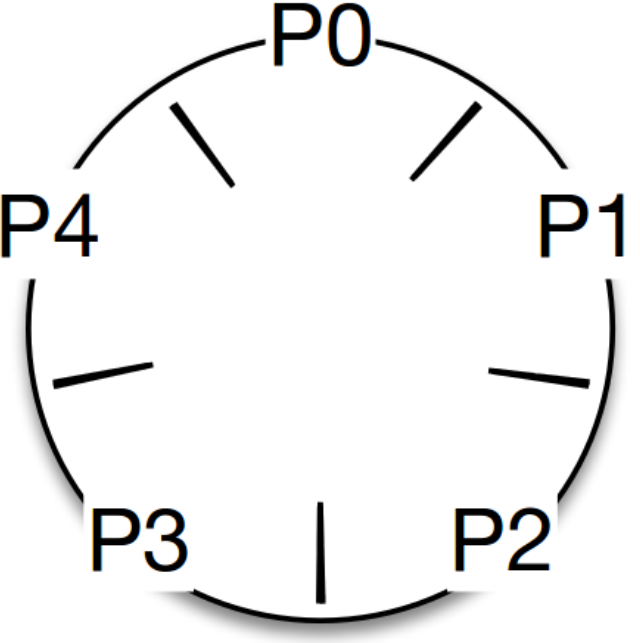
\includegraphics[width=0.25\textwidth]{fig/dining-phil.png}
%  \caption{Dining Philosophers}
%\end{figure}

%%
%%\sc{TODO: give example of data invariants}
%%
%%\sc{TODO: there exists a tool, Daikon, to detect these invariants for sequential systems}
%%
%%\sc{TODO: this paper introduces a similar tool to Daikon, but for distributed systems}
%%
%%\sc{TODO: this is different from prior work because the focus is on data affected by communication, and the introducing the concept of consistent distributed state; TODO: find related work of viewing distributed processing as sequential processing.}



